% =============================================================================
\section{The System}
\label{sec:system}
% =============================================================================

\textit{Lily} is a twin-thruster (differential-thrust) unmanned surface vehicle developed for autonomous survey and cooperative deploy/retrieve missions. The vehicle is controlled by a companion computer running ROS~2, bridged to a MAVLink autopilot (via \texttt{mavros}) that handles low-level attitude/position estimation, and interfaces with two brushless thrusters through VESC electronic speed controllers (ESCs) operating in Field-Oriented Control (FOC) mode.

\begin{figure}[ht!]
    \centering
    \includegraphics[width=\textwidth]{figures/bright_photo.jpg}
    \caption{The Lily USV, a twin-thruster autonomous surface vehicle.}
    \label{fig:lily}
\end{figure}

\subsection{Vehicle configuration and thruster layout}
\label{sec:hull}

The vehicle frame defines the sensor and actuator mounting points relative to \texttt{base\_link}, summarized in Table~\ref{tab:frames} and Figure~\ref{fig:layout}.

\begin{table}[H]
\centering
\caption{Sensor and actuator mounting offsets relative to \texttt{base\_link} (meters).}
\label{tab:frames}
\begin{tabular}{@{}llccc@{}}
\toprule
Frame & Component & $x$ [m] & $y$ [m] & $z$ [m] \\
\midrule
\texttt{left\_engine\_link}  & Port thruster      & $-0.80$ & $+0.33$ & $-0.15$ \\
\texttt{right\_engine\_link} & Starboard thruster & $-0.80$ & $-0.33$ & $-0.15$ \\
\texttt{lidar\_sensor}       & 3D LiDAR           & $+1.00$ & $0.00$  & $+0.70$ \\
\texttt{camera\_sensor}      & Monocular camera   & $+1.20$ & $0.00$  & $+0.70$ \\
\bottomrule
\end{tabular}
\end{table}

The two thrusters are mounted symmetrically about the centerline at the stern, giving a thruster (skid-steer) baseline of
\begin{equation}
L \;=\; y_{\text{left}} - y_{\text{right}} \;=\; 0.33 - (-0.33) \;=\; 0.66\ \text{m},
\end{equation}
which is exactly the \texttt{wheel\_base} parameter ($0.66$~m) used throughout the control stack (Section~\ref{sec:vw}). \todored{Confirm overall hull length/beam/draft and dry mass -- the URDF only encodes frame offsets, not the hull geometry. The velocity-controller comment in \texttt{velocity\_controller\_real.yaml} notes an estimated mass $\approx 42$\,kg and yaw inertia $I_z \approx 26\,\text{kg}\,\text{m}^2$; confirm/replace with measured values.}

\begin{figure}[H]
\centering
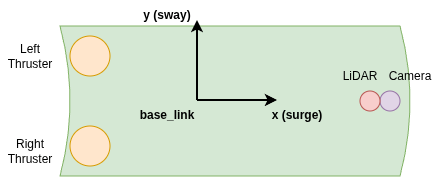
\includegraphics[width=0.7\textwidth]{figures/esquema.drawio.png}
\caption{Vehicle layout and sensor/actuator mounting points.}
\label{fig:layout}
\end{figure}

\subsection{Compute and communications architecture}

Figure~\ref{fig:arch} shows the software architecture. The companion computer runs ROS~2 nodes for guidance, control and perception; \texttt{mavros} bridges MAVLink telemetry commands to and from the autopilot; the autopilot performs attitude and position estimation and redirects RC input, arming and mode services.

\begin{figure}[H]
\centering
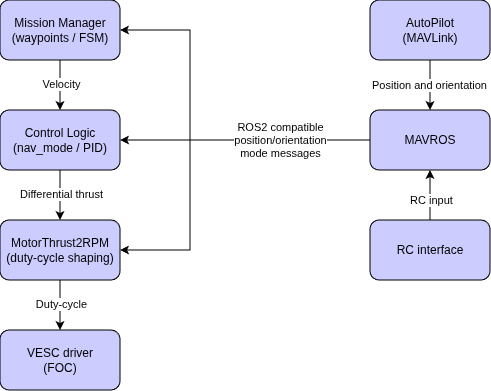
\includegraphics[width=0.7\textwidth]{figures/esquema2.drawio.png}
\caption{Software architecture.}
\label{fig:arch}
\end{figure}

\subsection{Localization and State Estimation}
\label{sec:localization}

The vehicle's pose and velocity feedback, used by all high-level control systems, rely on an Extended Kalman Filter (EKF) running natively on the autopilot's onboard firmware. Rather than computing state estimates within the external companion computer workspace, the higher-level control architecture acts purely as a consumer of the autopilot's telemetry. 

The onboard EKF operates as a black-box state estimator, fusing two primary sensor streams:
\begin{itemize}
    \item \textbf{High-rate Inertial Measurement Unit (IMU) data:} Providing angular rate and linear acceleration. For this 3~DoF Unmanned Surface Vehicle (USV), the critical components are planar accelerations and yaw rate. 
    \item \textbf{Global Navigation Satellite System (GNSS/GPS) data:} Supplying raw global positioning fixes.
\end{itemize}

By fusing these inputs, the EKF produces a stabilized, continuous odometry signal containing the vehicle's fused pose and velocity (twist). This finalized estimate is the sole feedback signal driving the vehicle's control logic, velocity regulation, and mission management. 

To map the global GPS data into a usable Cartesian space for 3~DoF planar control, a local East-North-Up (ENU) datum is established at the beginning of each operational session. In simulation environments, this origin is automatically parsed from the simulated world's configuration, whereas on the physical vehicle, it is initialized by the autopilot upon arming. Once this local datum is set, the mission manager converts all global geodetic waypoints (latitude and longitude) into local ENU coordinates using a flat-Earth approximation. This allows the USV to navigate using standard planar geometry relative to its starting location.

\begin{center}
\rednote{Should we dive into the EKF formulation (state vector, prediction/correction equations), or just describe that we used the ArduSub/ArduPilot on-board EKF as-is, without re-deriving it here?}
\end{center}

\todored{Confirm which autopilot firmware and EKF (e.g. ArduPilot EKF3, PX4 EKF2) Lily actually runs, and, if we do decide to elaborate, paste in the actual noise/process covariance tuning (\texttt{EK3\_*} or \texttt{EKF2\_*} parameters) so the description is vehicle-specific rather than generic.}
